\section*{Step 2}

\begin{custombox}[label={box:Q2}]{Step 2}
	Review the data using appropriate plots and understand the overall structure of the data. Comment on the data and anticipate how well \texttt{LogisticRegression} will perform on the data.
\end{custombox}

This is how I plotted the 3 datasets

\begin{lstlisting}[language=Python, caption=Plotting the Datasets]
datasets = [(data_v0, "Dataset 1"), 
            (data_v1, "Dataset 2"),
            (data_v2, "Dataset 3")]

for i, (data, label) in enumerate(datasets):
    plt.figure(figsize=(16, 10))
    
    plt.scatter(data['x1'], data['x2'], c=data['y'], cmap='viridis', s=10)
    plt.title(f'Scatter Plot of {label}')
    plt.xlabel('x1')
    plt.ylabel('x2')
    
    plt.tight_layout()
    plt.savefig(f'Images/dataset-{i+1}-overview.png', dpi=400)
    plt.show()
    
    class_counts = data['y'].value_counts()
    print(f"Class balance in {label}:\n{class_counts}\n")
\end{lstlisting}

\begin{figure}[H]
    \centering
    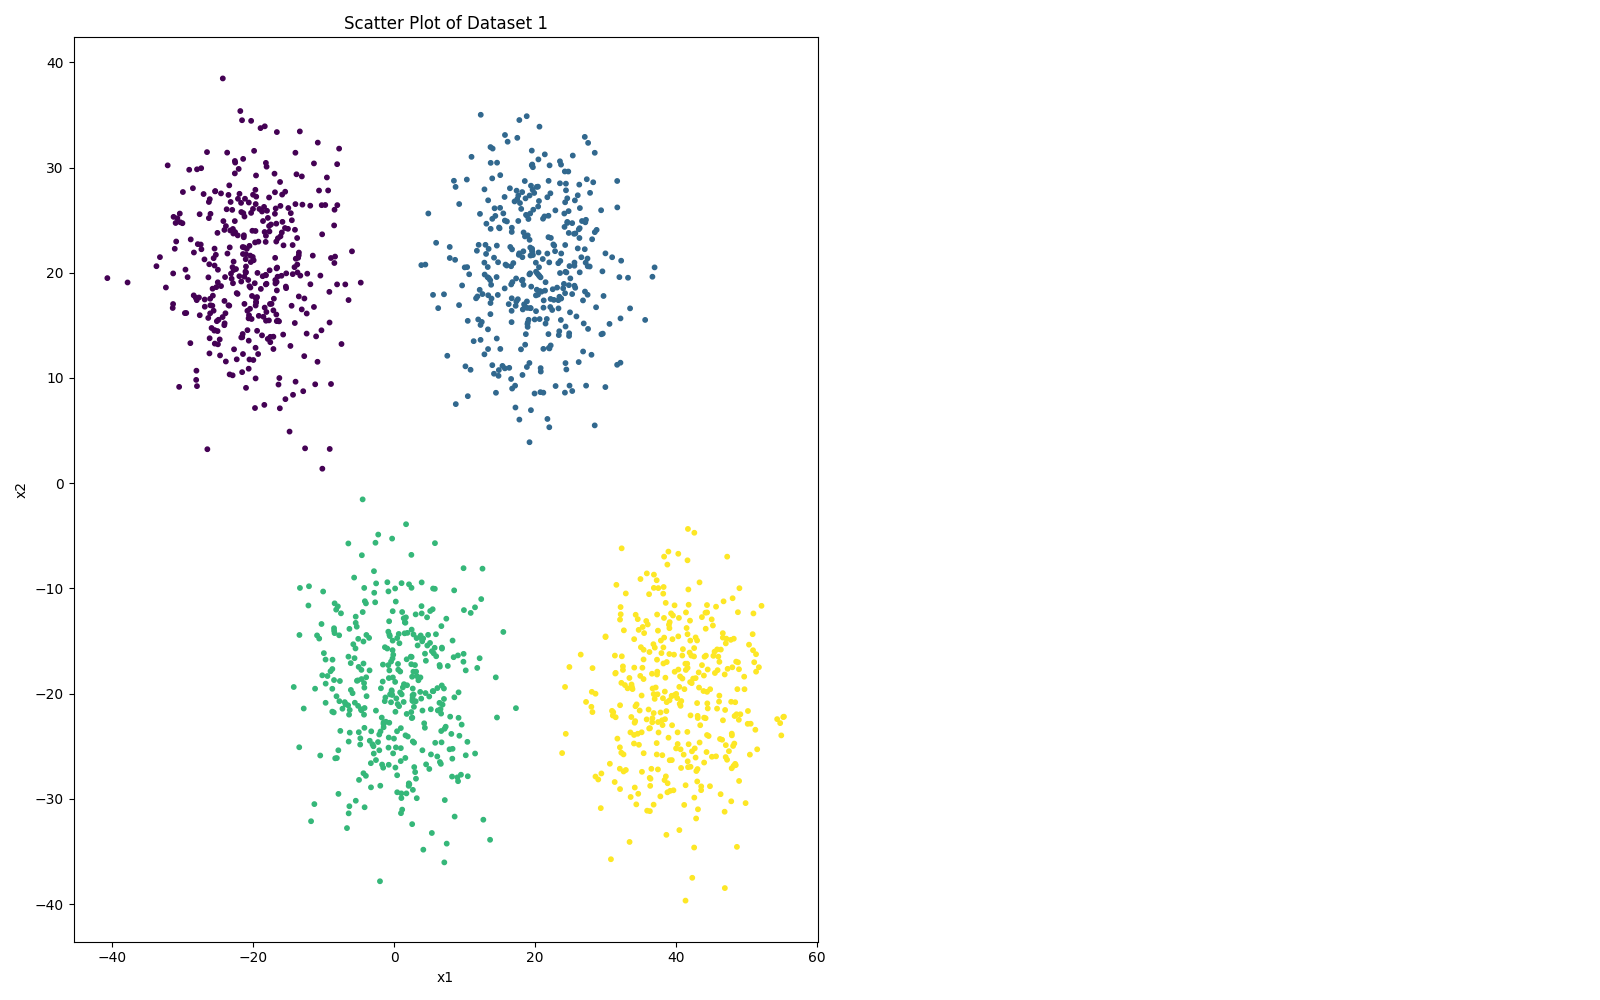
\includegraphics[width=0.7\textwidth]{Images/dataset-1-overview.png}
    \caption{Overview of Data Set 1}
\end{figure}

\begin{figure}[H]
    \centering
    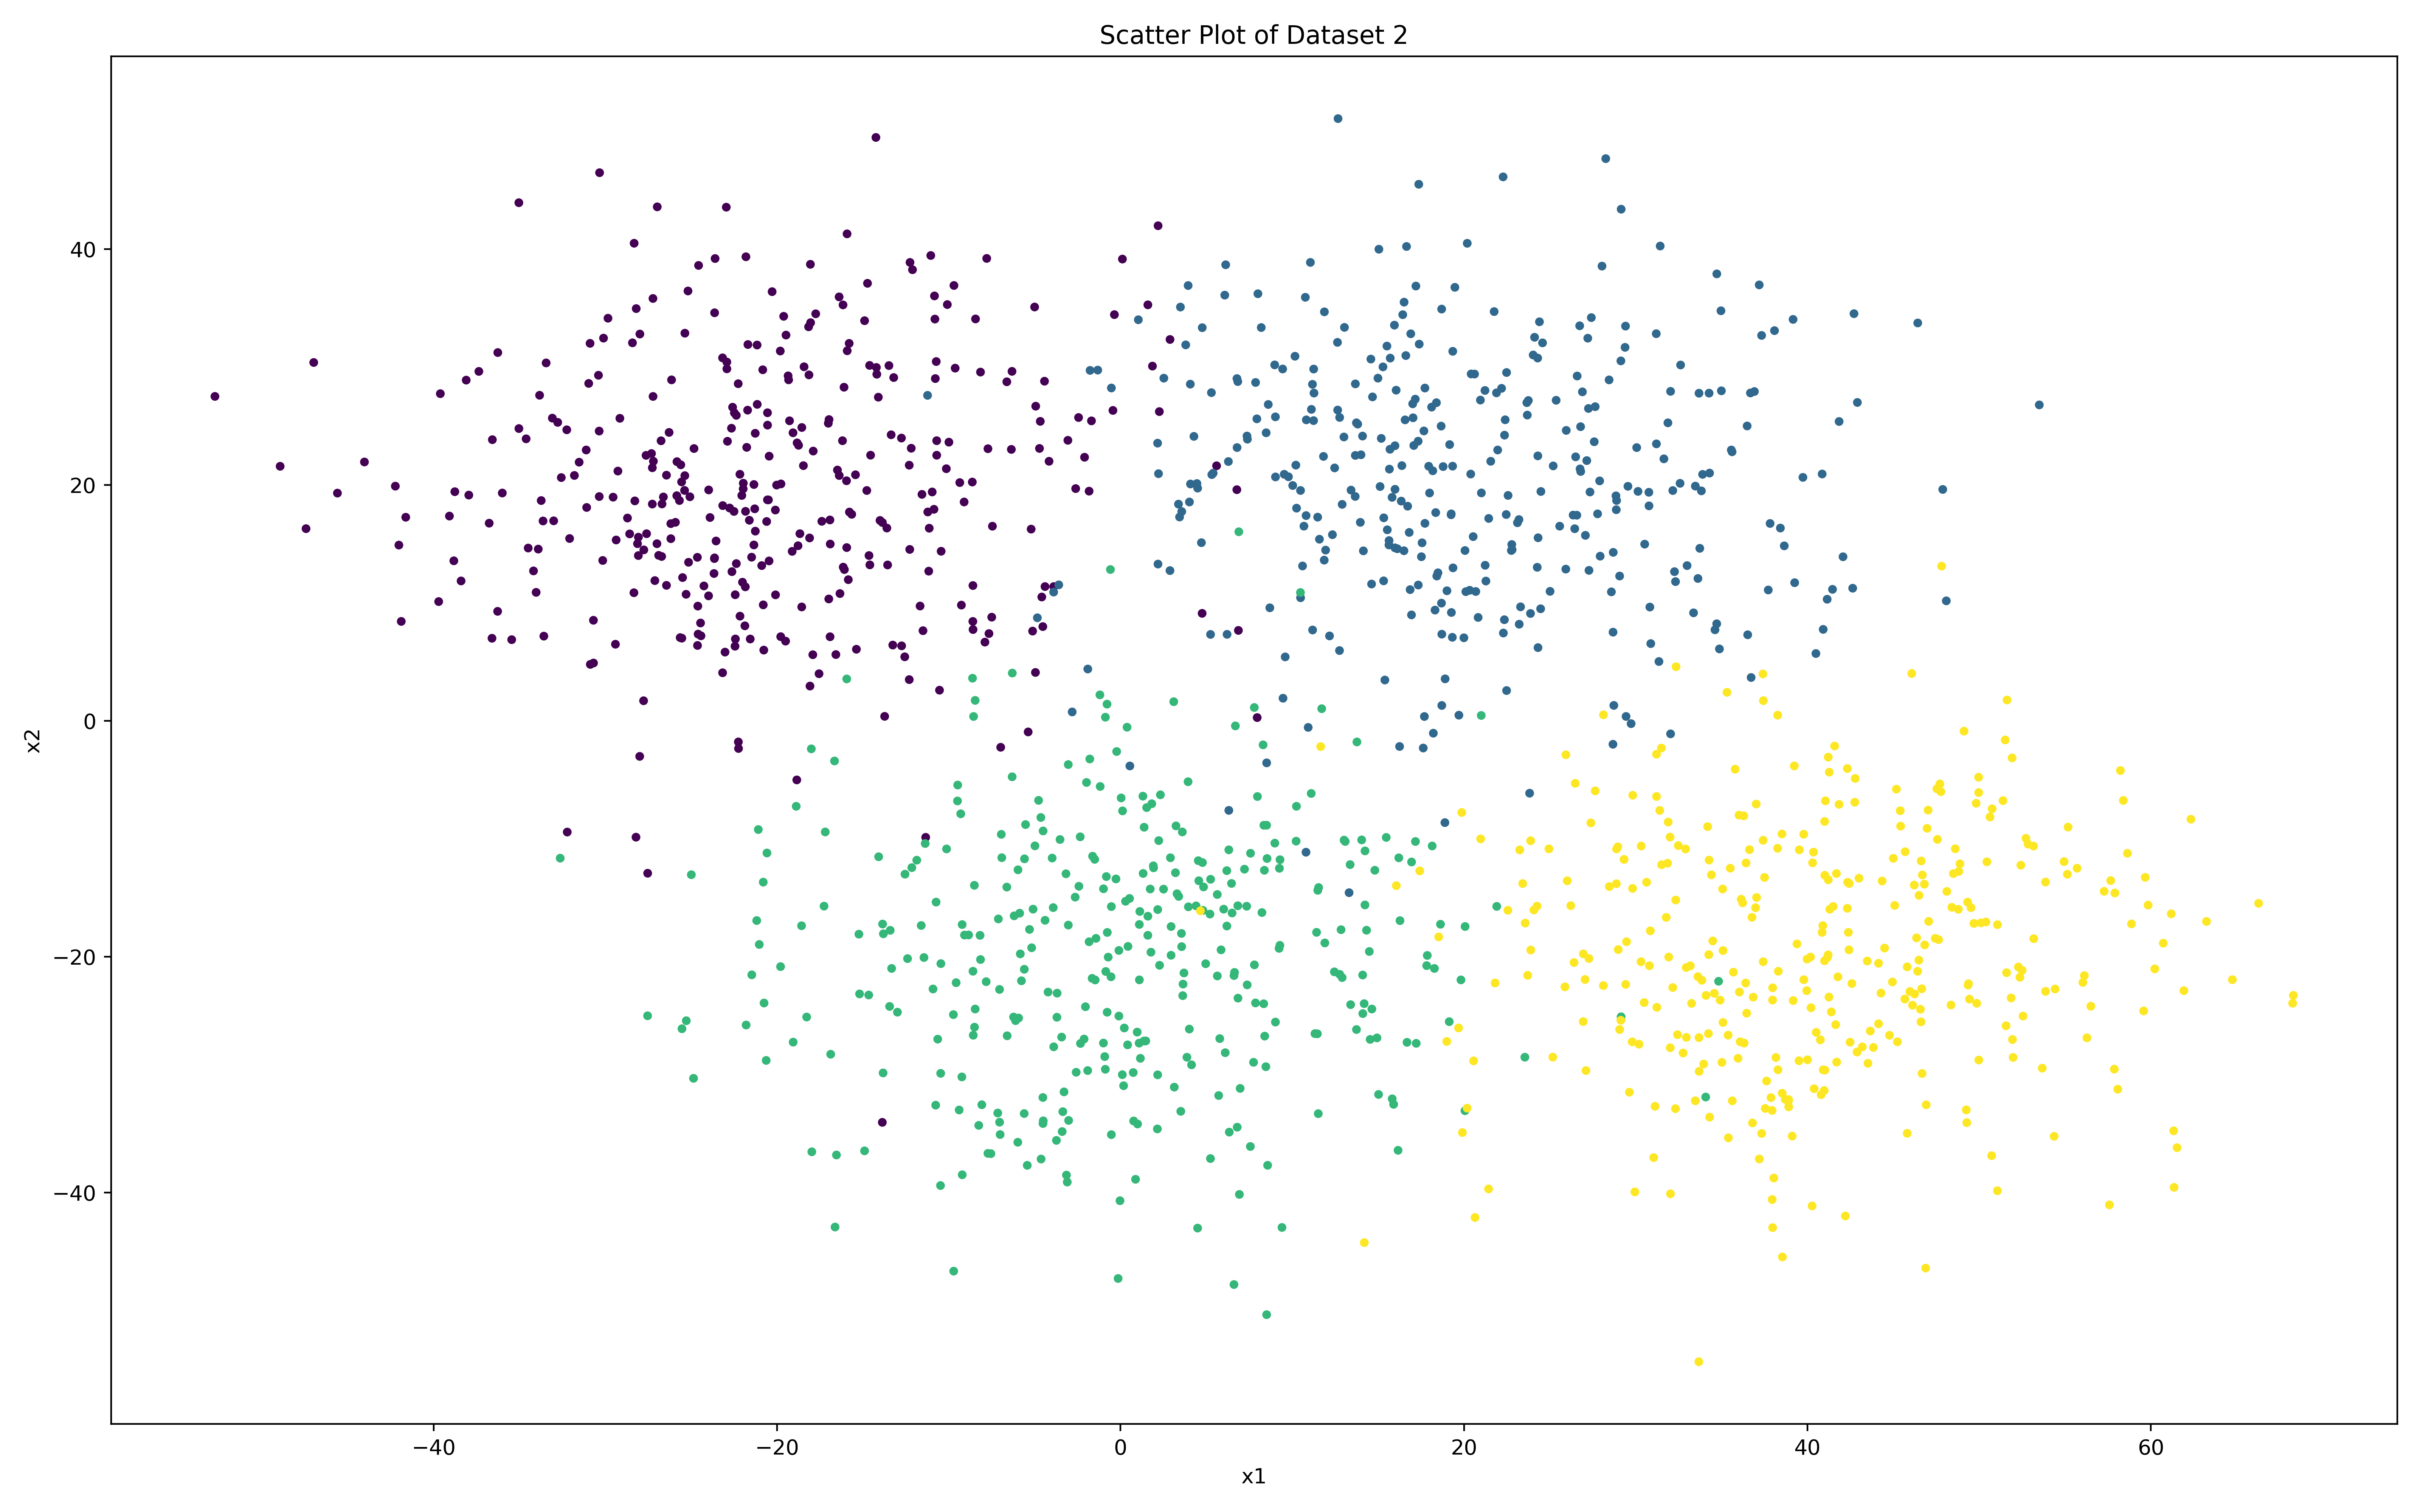
\includegraphics[width=0.7\textwidth]{Images/dataset-2-overview.png}
    \caption{Overview of Data Set 2}
\end{figure}

\begin{figure}[H]
    \centering
    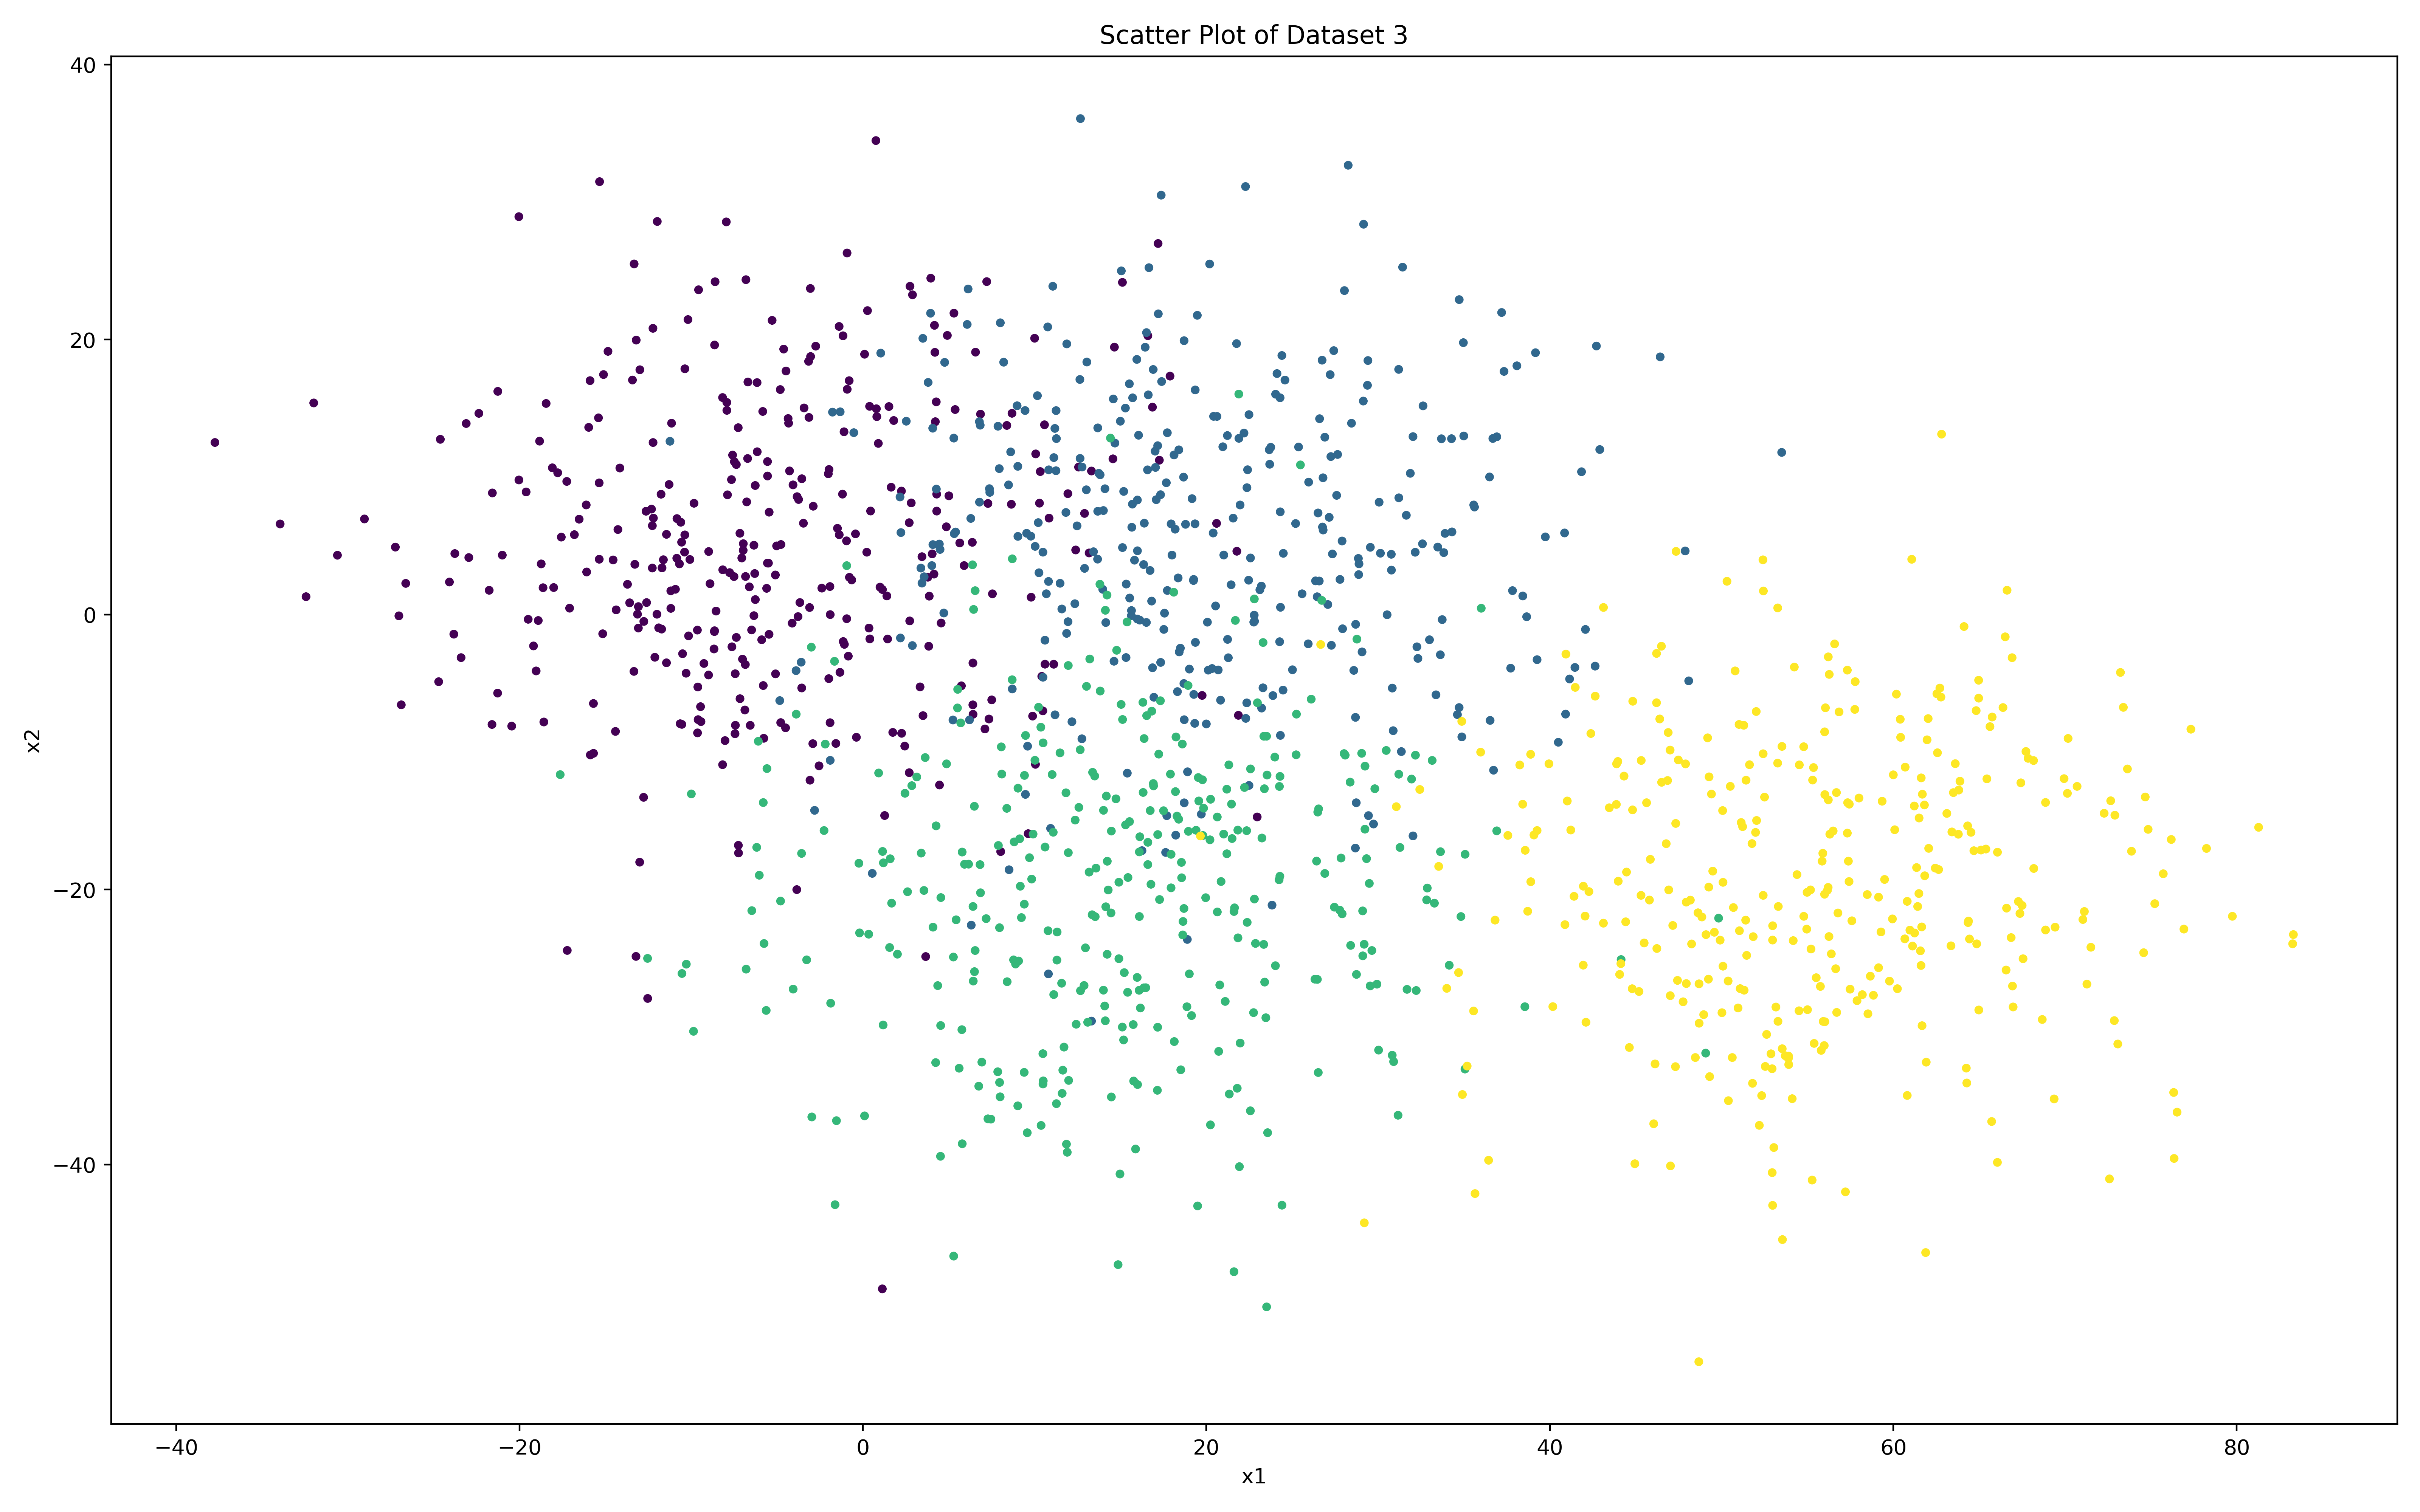
\includegraphics[width=0.7\textwidth]{Images/dataset-3-overview.png}
    \caption{Overview of Data Set 3}
\end{figure}

We see that in each dataset, there are $360$ points. The data is balanced in all the datasets. The data in Dataset $1$ is linearly separable, the data in Dataset $2$ is not linearly separable, and the data in Dataset $3$ is more complex than the data in Dataset $2$.

This is how I plotted the training and testing datasets.

\begin{lstlisting}[language=Python, caption=Plotting the Training and Testing Datasets]
plt.figure(figsize=(16, 6))
plt.subplot(1, 2, 1)
plt.scatter(x_train_v0['x1'], x_train_v0['x2'], c=y_train_v0, cmap='viridis', s=10)
plt.title('Training data for Dataset 1')

plt.subplot(1, 2, 2)
plt.scatter(x_test_v0['x1'], x_test_v0['x2'], c=y_test_v0, cmap='viridis', s=10)
plt.title('Test data for Dataset 1')
plt.savefig('Images/dataset-1-train-test.png', dpi=400)
plt.show()

plt.figure(figsize=(16, 6))
plt.subplot(1, 2, 1)
plt.scatter(x_train_v1['x1'], x_train_v1['x2'], c=y_train_v1, cmap='viridis', s=10)
plt.title('Training data for Dataset 2')

plt.subplot(1, 2, 2)
plt.scatter(x_test_v1['x1'], x_test_v1['x2'], c=y_test_v1, cmap='viridis', s=10)
plt.title('Test data for Dataset 2')
plt.savefig('Images/dataset-2-train-test.png', dpi=400)
plt.show()

plt.figure(figsize=(16, 6))
plt.subplot(1, 2, 1)
plt.scatter(x_train_v2['x1'], x_train_v2['x2'], c=y_train_v2, cmap='viridis', s=10)
plt.title('Training data for Dataset 3')

plt.subplot(1, 2, 2)
plt.scatter(x_test_v2['x1'], x_test_v2['x2'], c=y_test_v2, cmap='viridis', s=10)
plt.title('Test data for Dataset 3')
plt.savefig('Images/dataset-3-train-test.png', dpi=400)
plt.show()
\end{lstlisting}

\clearpage

This is how the test and train datasets look for each data set.

\begin{figure}[H]
    \centering
    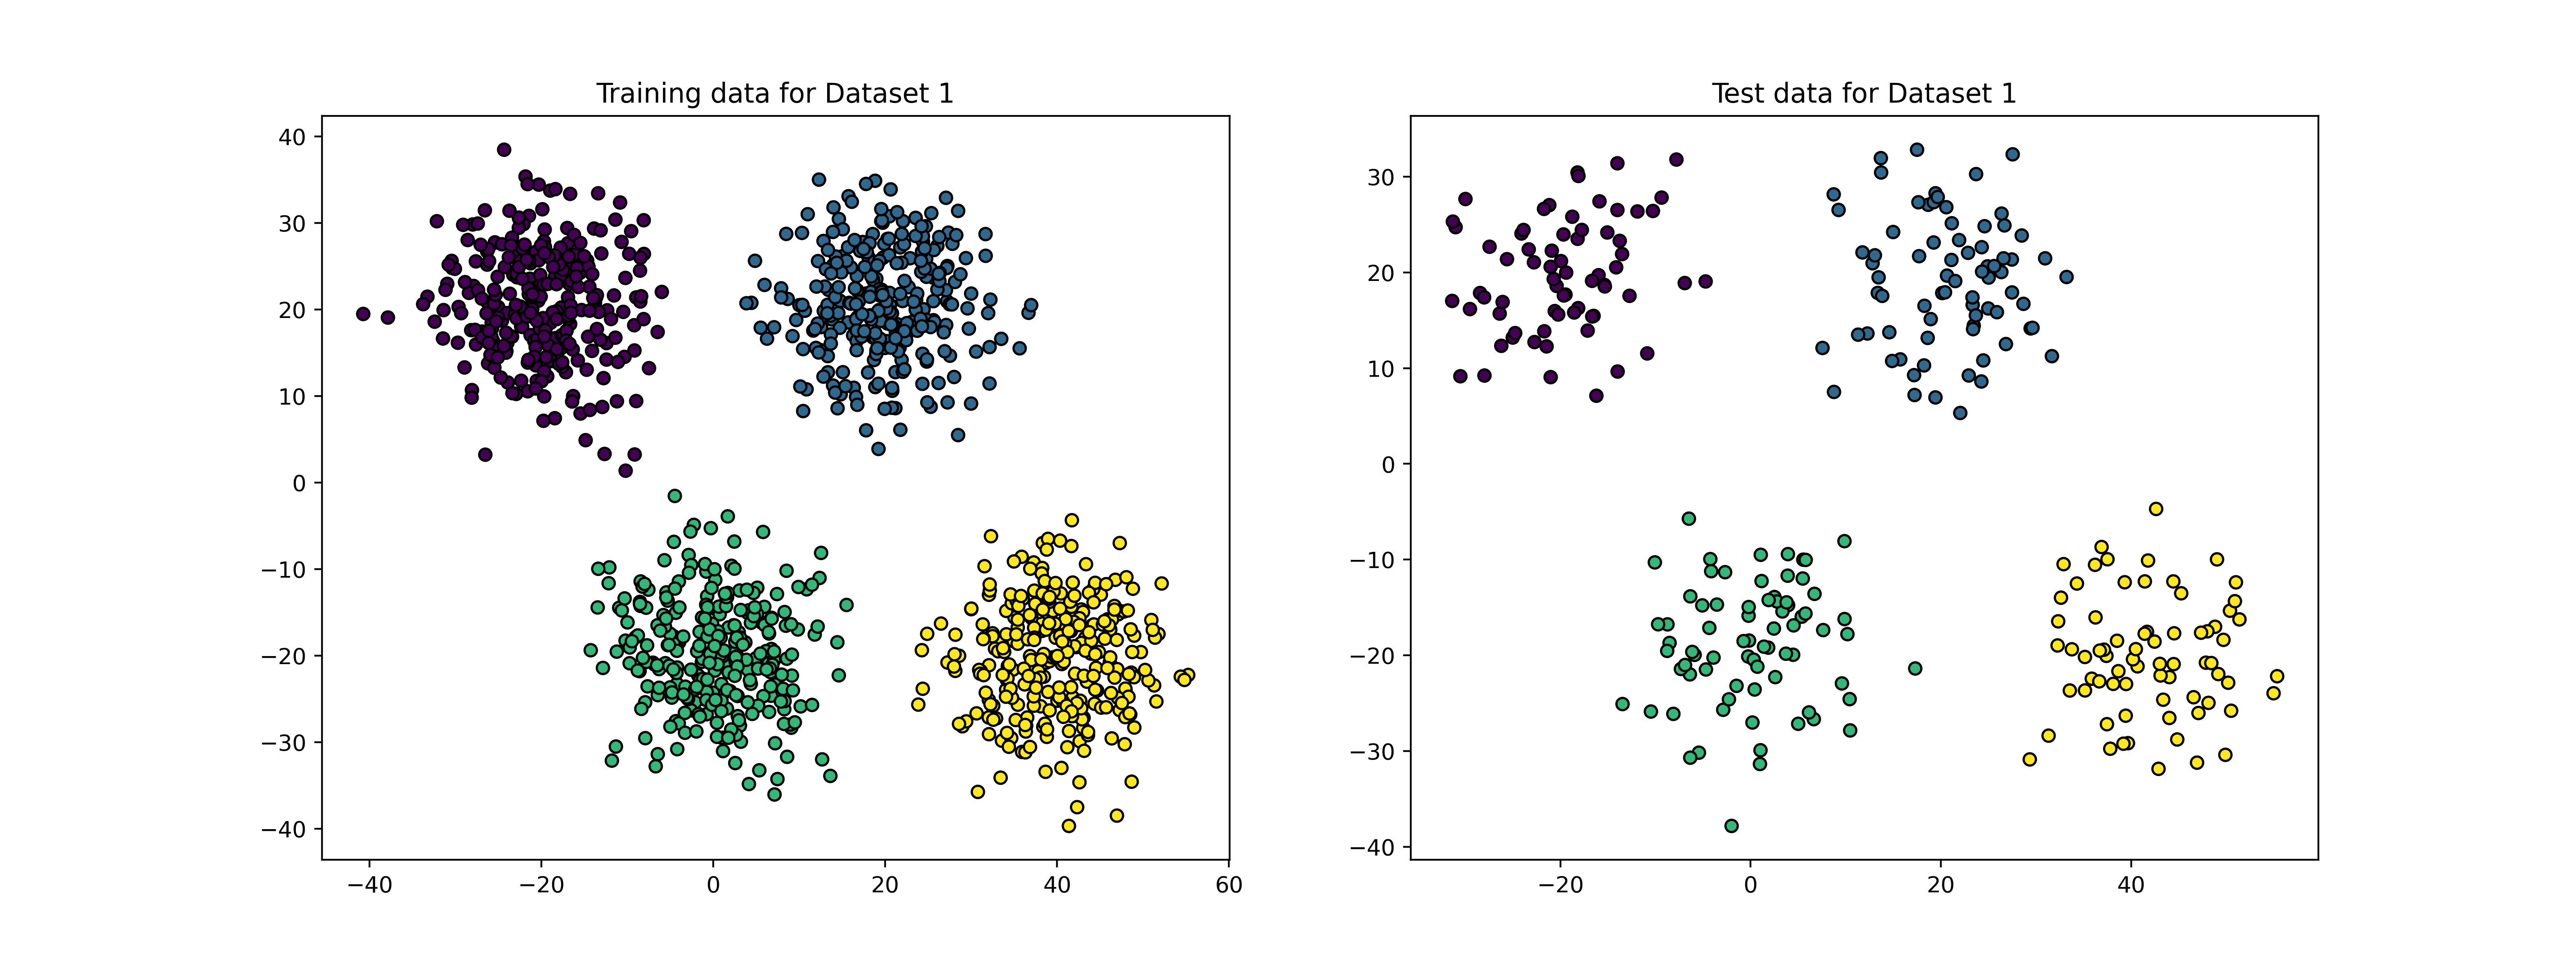
\includegraphics[width=0.9\textwidth]{Images/dataset-1-train-test.png}
    \caption{Training and Testing Datasets for Data Set 1}
\end{figure}

\begin{figure}[H]
    \centering
    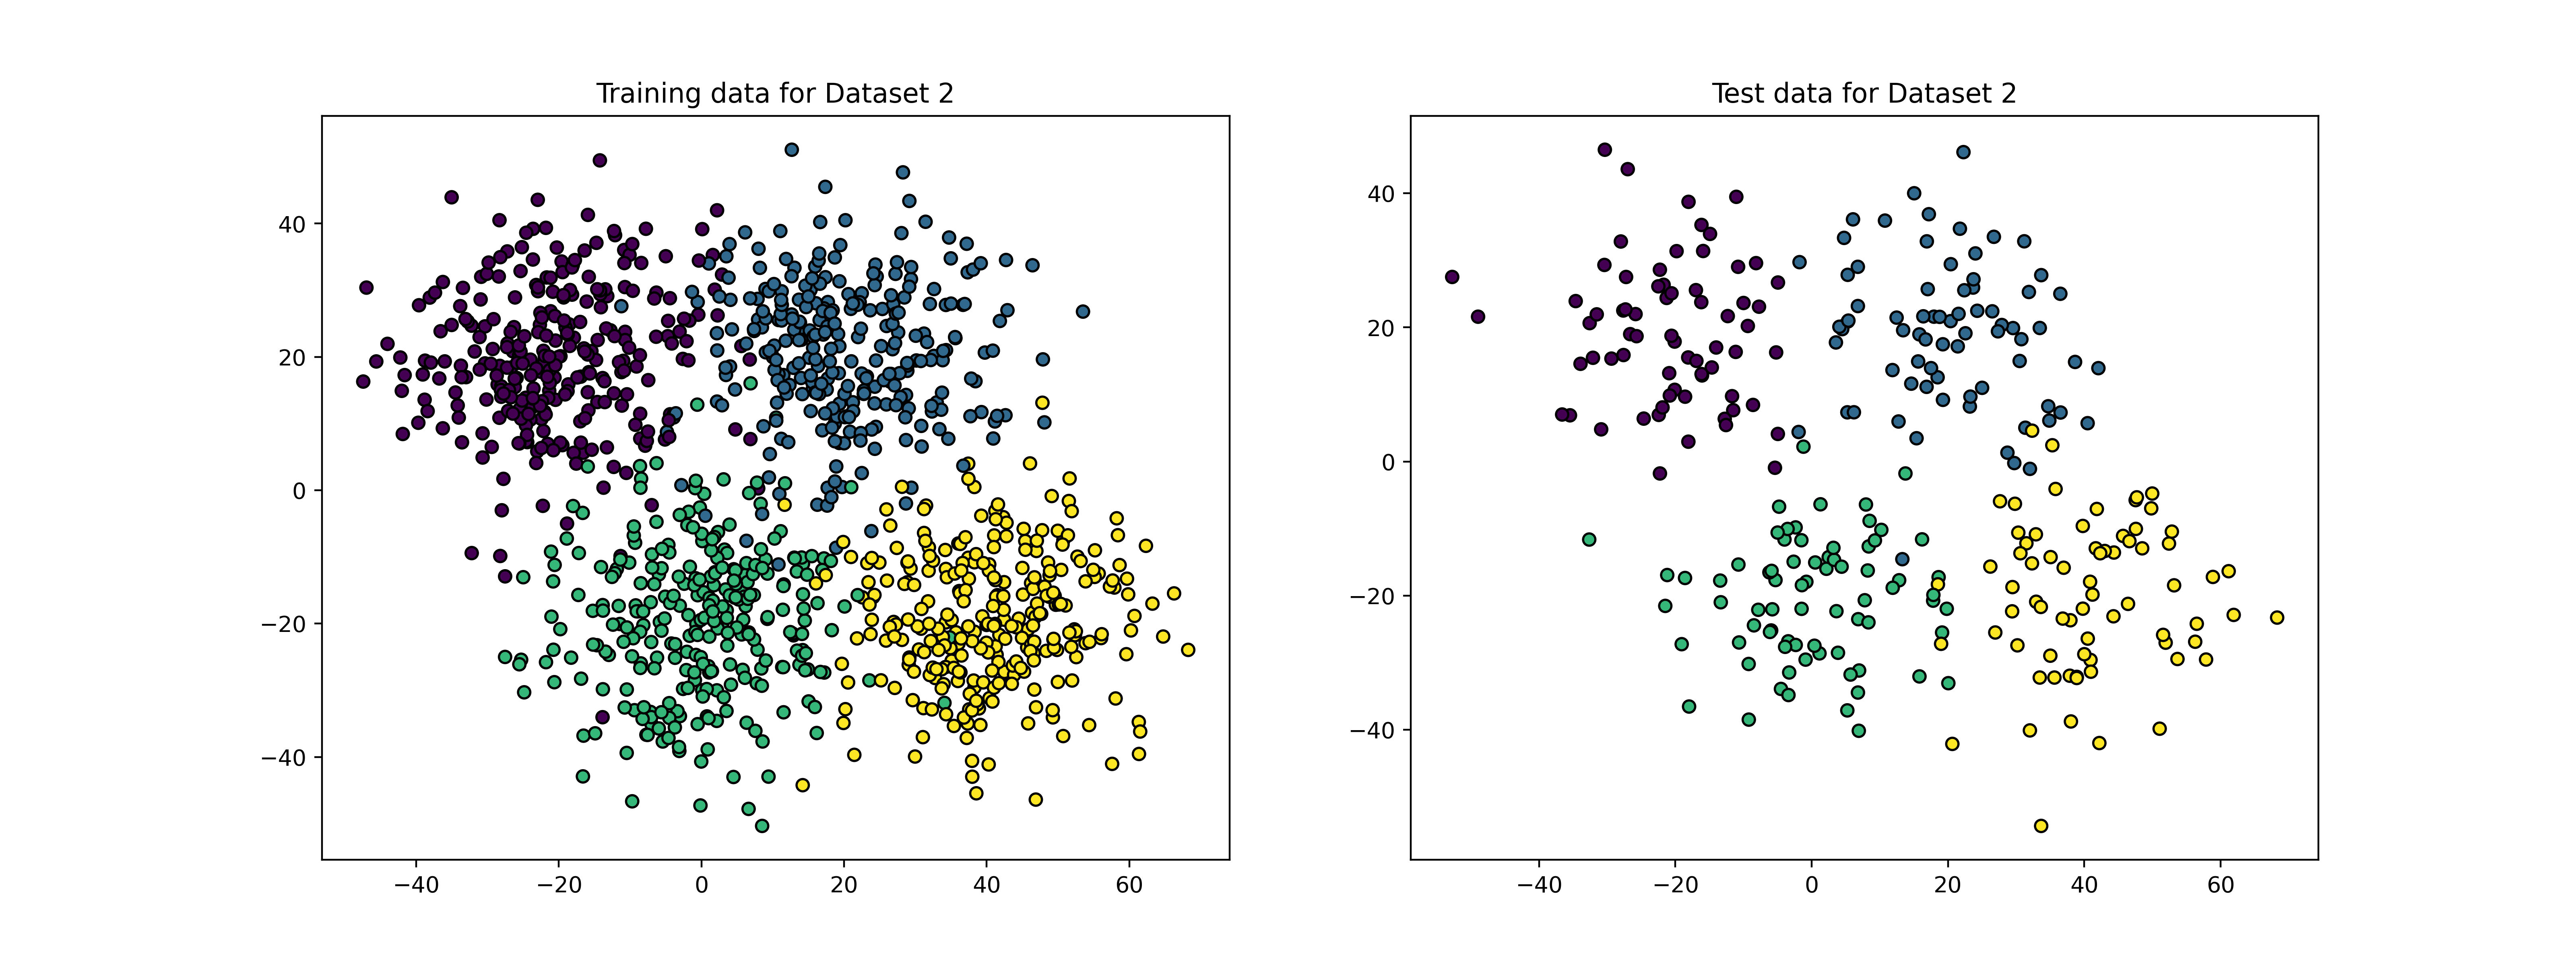
\includegraphics[width=0.9\textwidth]{Images/dataset-2-train-test.png}
    \caption{Training and Testing Datasets for Data Set 2}
\end{figure}

\begin{figure}[H]
    \centering
    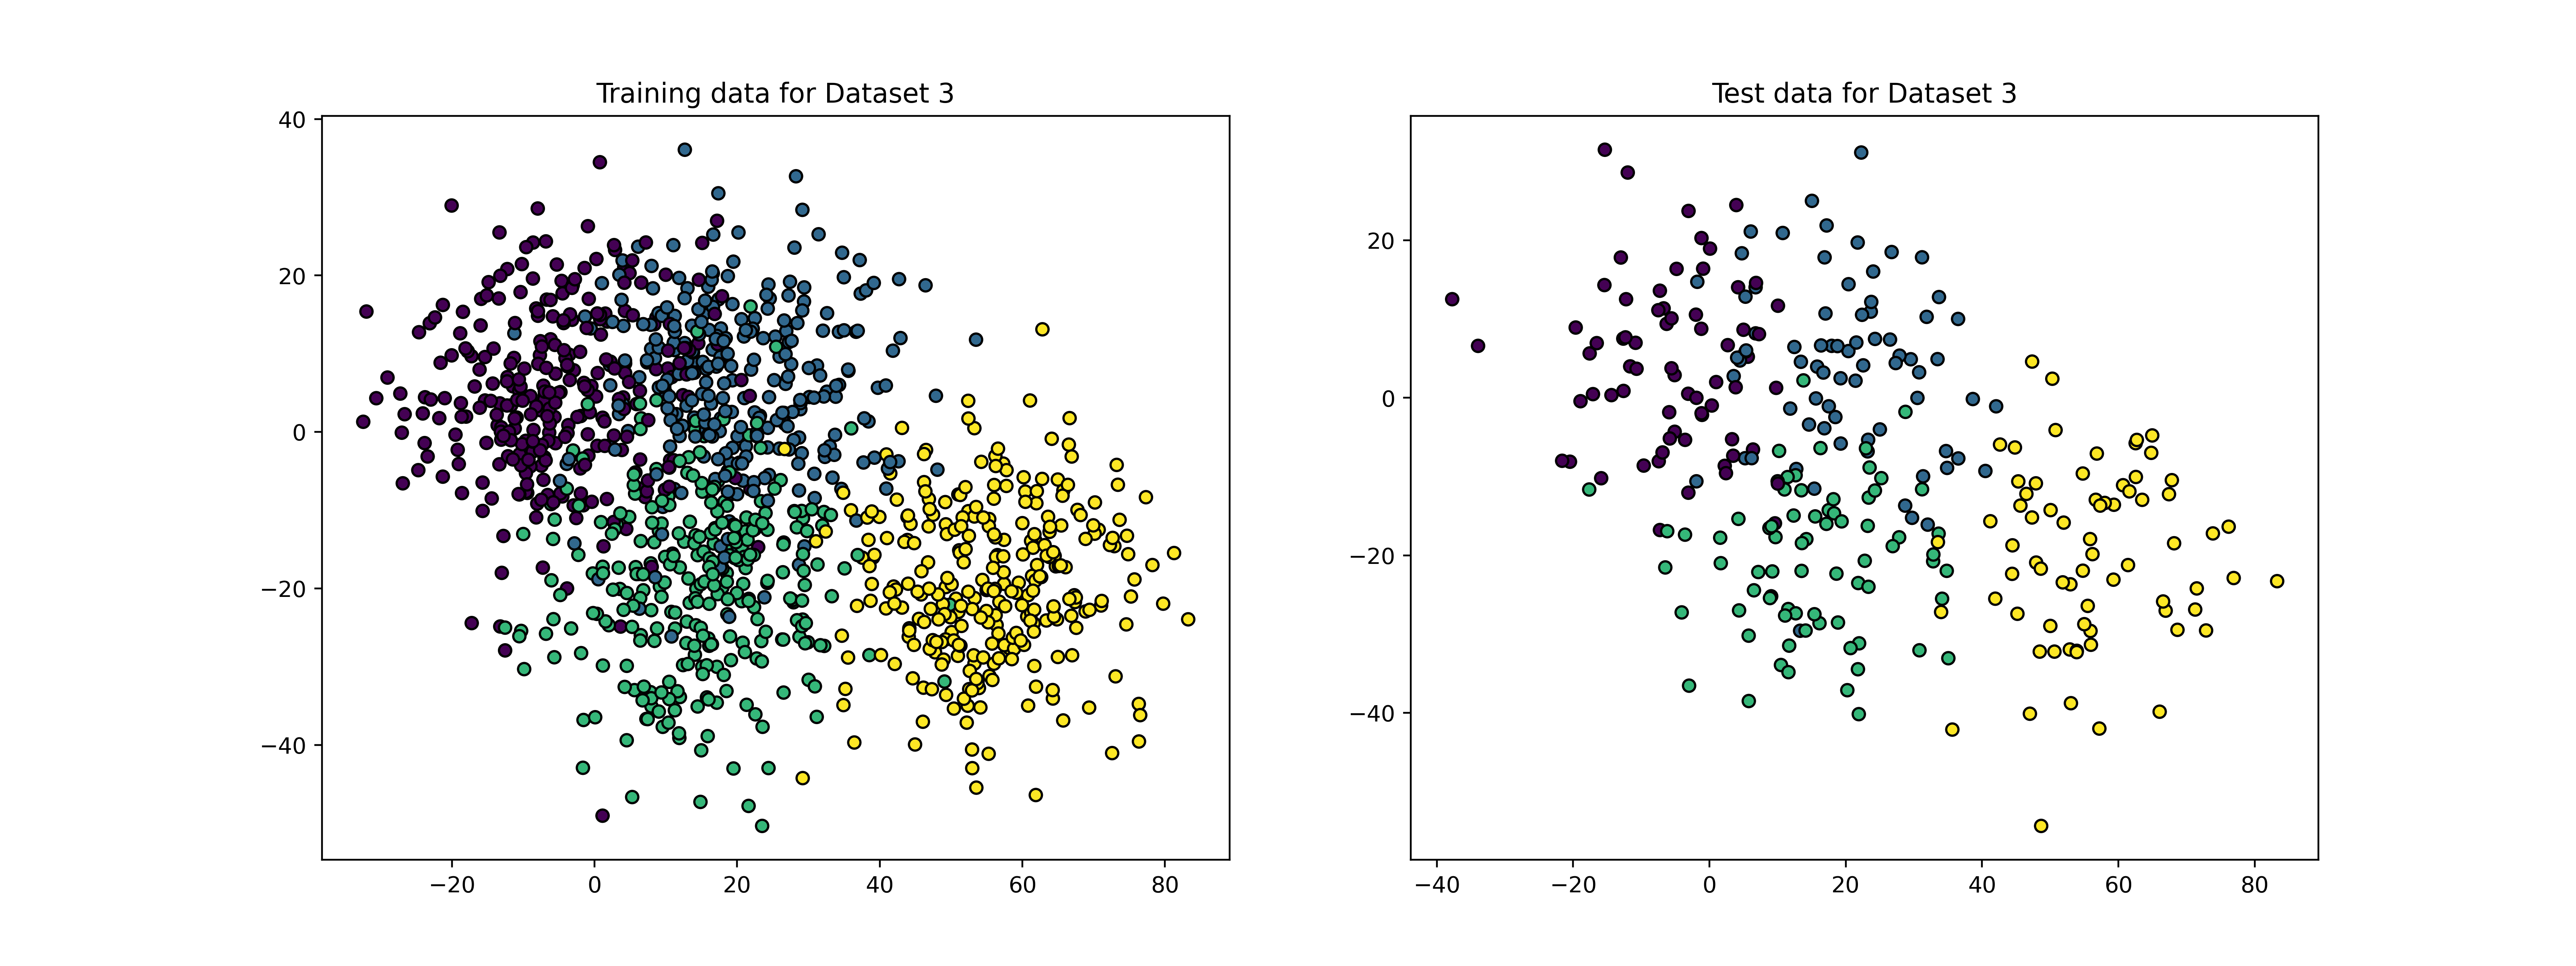
\includegraphics[width=0.9\textwidth]{Images/dataset-3-train-test.png}
    \caption{Training and Testing Datasets for Data Set 3}
\end{figure}

\clearpage

Reviewing the plots above, we can see that the training data and the test data are well balanced in all the $3$ situations. The data is somewhat linearly separable in Dataset $1$, but not so much in Dataset $2$ and Dataset $3$. The data in Dataset $3$ is more complex than in Dataset $2$.

Logistic Regression will perform well on Dataset $1$ as it is linearly separable. It will perform poorly on Dataset $2$ and Dataset $3$ as they are not linearly separable. We can expect that the model will have a high accuracy on Dataset $1$ and a low accuracy on Dataset $2$ and Dataset $3$.




